\chapter{Appendix 1} \label{app:whitening}

\begin{figure}[h!t]
	\begin{center}
		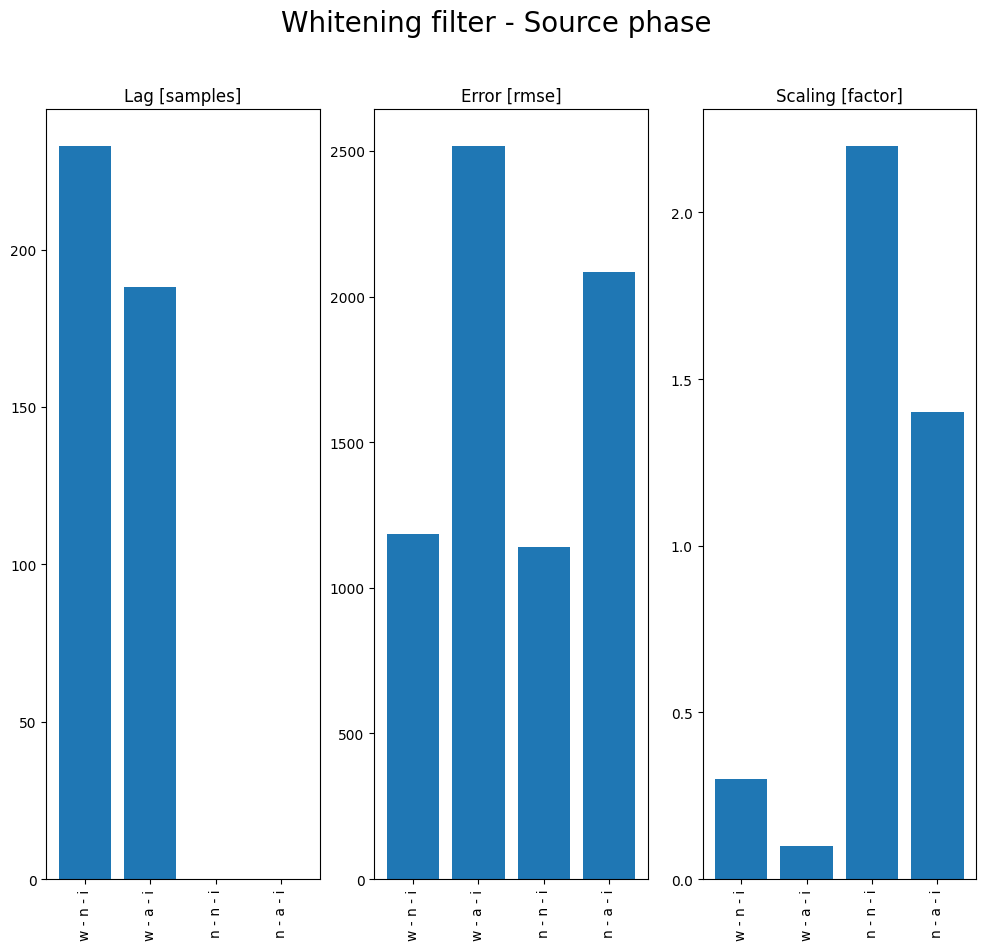
\includegraphics[width=1.0\columnwidth]{images/result_whitening_sourcephase.png}
	\end{center}
	\caption{Lag, error, and scaling of different filtering and envelope techniques with whitening applied. The whitening filter is constructed from the desired frequency amplitude response and a phase. The frequency response is determined as described in the simulation section \ref{sec:whitening}, and the phase is set to the phase of the input signal that was used to construct the whitening filter. }
	\label{fig:result_whitening_sourcephase}
\end{figure}

\begin{figure}[h!t]
	\begin{center}
		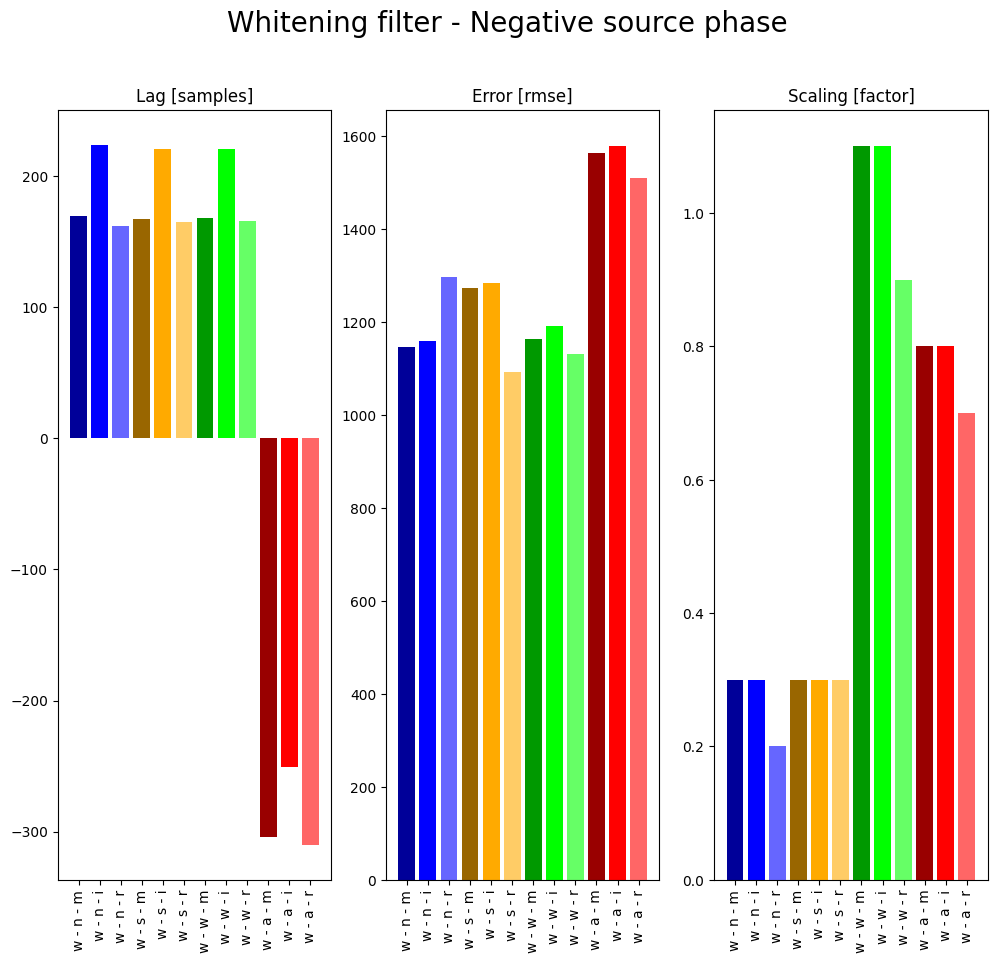
\includegraphics[width=1.0\columnwidth]{images/result_whitening_negative_sourcephase.png}
	\end{center}
	\caption{Lag, error, and scaling of different filtering and envelope techniques with whitening applied. The whitening filter is constructed from the desired frequency amplitude response and a phase. The frequency response is determined as described in the simulation section \ref{sec:whitening}, and the phase is set to the negative phase of the input signal that was used to construct the whitening filter. }
	\label{fig:result_whitening_negative_sourcephase}
\end{figure}

\begin{figure}[h!t]
	\begin{center}
		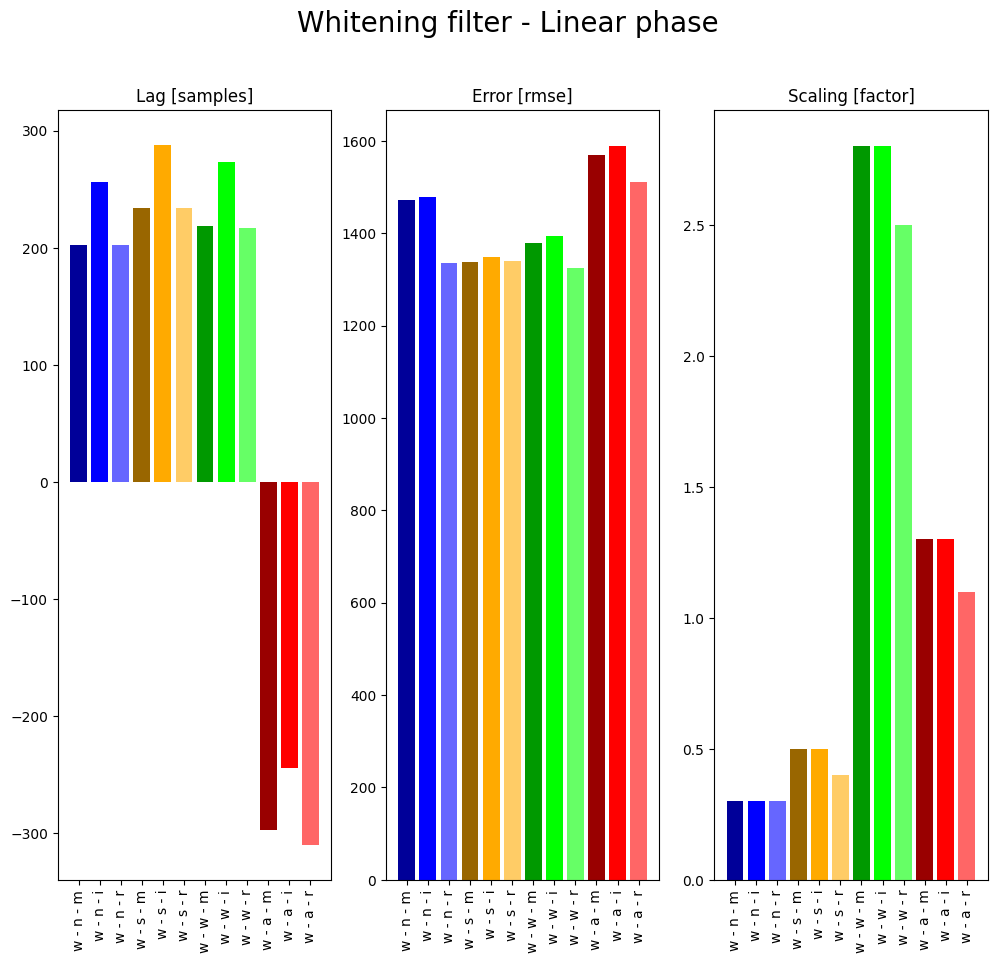
\includegraphics[width=1.0\columnwidth]{images/result_whitening_linearphase.png}
	\end{center}
	\caption{Lag, error, and scaling of different filtering and envelope techniques with whitening applied. The whitening filter is constructed from the desired frequency amplitude response and a phase. The frequency response is determined as described in the simulation section \ref{sec:whitening}, and the phase is set to linear phase. }
	\label{fig:result_whitening_linearphase}
\end{figure}

\begin{figure}[h!t]
	\begin{center}
		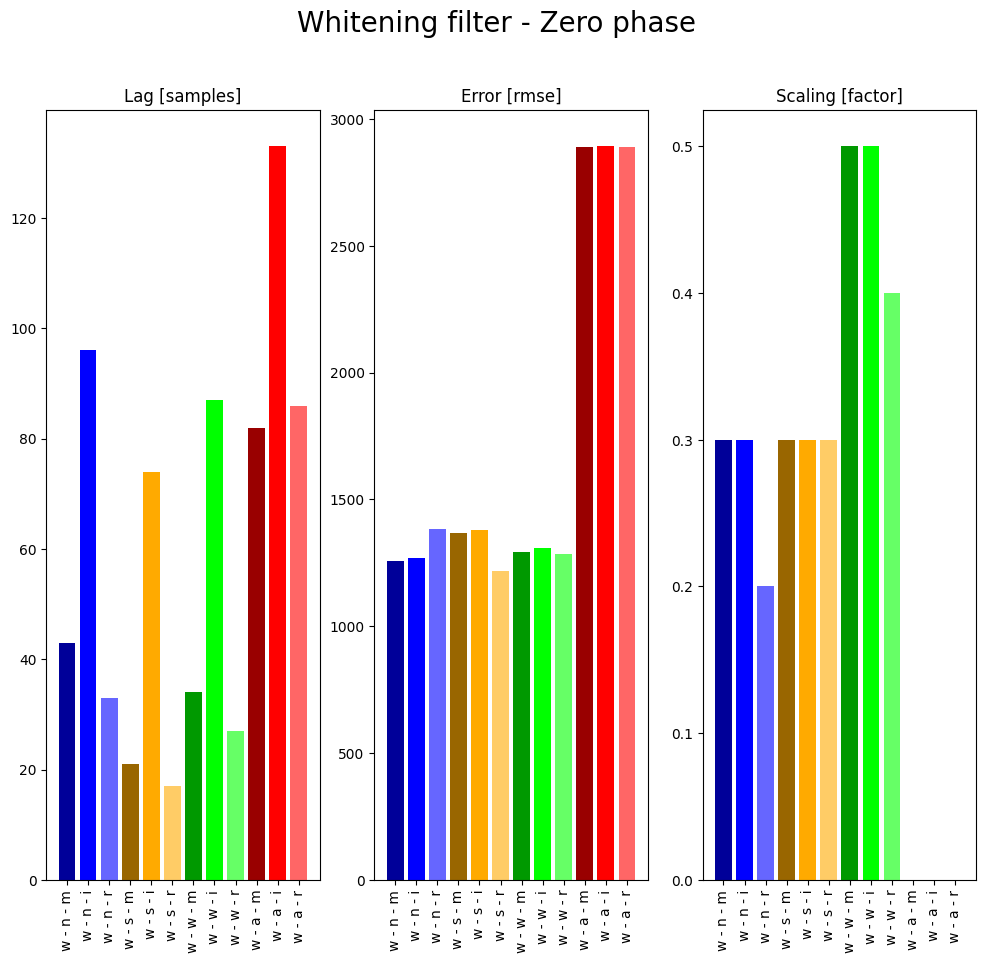
\includegraphics[width=1.0\columnwidth]{images/result_whitening_zerophase.png}
	\end{center}
	\caption{Lag, error, and scaling of different filtering and envelope techniques with whitening applied. The whitening filter is constructed from the desired frequency amplitude response and a phase. The frequency response is determined as described in the simulation section \ref{sec:whitening}, and the phase is set to zero phase. }
	\label{fig:result_whitening_zerophase}
\end{figure}